\documentclass[compress]{beamer}
\usepackage[utf8]{inputenc}  
\usepackage[francais]{babel}
\usetheme{Warsaw}
\usepackage[T1]{fontenc}
\usepackage[]{bbm}
\usepackage{amsfonts}
\usepackage{amsmath}
\usepackage{amssymb}
\usepackage{amsthm}
\usepackage{graphicx}
\usepackage{pstricks}
\usepackage{float}
\usepackage[autolanguage]{numprint}
%\usepackage[squaren,Gray]{SIunits}
\usepackage{tikz}
\usepackage[size=A4]{beamerposter}%
%\usepackage{multimedia}
	
\title{Cryptography and its relevance in today's world}
\subtitle{Fighting back against global surveillance}
\author{}
\date{}

\newcommand{\sgn}{ \mathop{\textrm{sgn}}}
\renewcommand{\le}{\leqslant}
\renewcommand{\ge}{\geqslant}
\newcommand{\et}{\textrm{ et }}
\newcommand{\ou}{\textrm{ ou }}
\newcommand{\de}{\textrm{ de }}
\newcommand{\si}{\textrm{ si }}
\newcommand{\E}{\mathcal{E}}
\newcommand{\V}{\vect{\mathcal{V}}}
\newcommand{\R}{\mathbb{R}}
\newcommand{\Z}{\mathbb{Z}}
\newcommand{\z}[1]{\Z/#1\Z}
\renewcommand{\P}{\mathbb{P}}
\newcommand{\Q}{\mathbb{Q}}
\newcommand{\N}{\mathbb{N}}
\newcommand{\C}{\mathbb{C}}
\newcommand{\K}{\mathbb{K}}
\newcommand{\f}{\widehat{f}}
\newcommand{\e}[1]{e^{-2 \pi i #1}}
\newcommand{\ex}[1]{e^{2 \pi i #1}}
\renewcommand{\L}[1]{L^{#1} (\R )}
	
\newcommand{\inte}[1]{\int_\mathbb{R} #1 \,d\lambda}
\newcommand{\intex}{\int_\mathbb{R}}
\newcommand{\dl}{d\lambda}
\newcommand{\conv}[2]{#1 \ast #2}
	
\newcommand{\vect}[1]{\overrightarrow{#1}}
\newcommand{\disp}[1]{\displaystyle{#1}}
	
\setcounter{secnumdepth}{3} %pour la numérotation subsubsection
\setcounter{tocdepth}{3} %pour la numérotation dans la table de matières
\renewcommand{\theenumi}{\roman{enumi})}
\renewcommand{\thesection}{\Roman{section}}
\renewcommand{\thesubsection}{\arabic{subsection}}
\renewcommand{\thesubsubsection}{\alph{subsubsection}}
	
\newcommand{\fonction}[5]{\begin{array}{cllll}
#1 & : & #2 & \longrightarrow & #3 \\
&    & #4 & \longmapsto & #5 \end{array}}
\newcommand{\fonc}[3]{\begin{array}{lllll}
#1: & #2 & \mapsto & \displaystyle{#3}\end{array}}
\newcommand{\app}[3]{
	#1 : #2 \mapsto \displaystyle{#3}}
\newcommand{\fonct}[3]{\begin{array}{ccccc}
#1: & #2 & \longrightarrow & \displaystyle{#3}\end{array}}
	
\newcommand{\ent}[2]{
	%\comp{#3}{\N}{#1\leqslant #3 \leqslant #2}
	[\![#1\,;\,#2]\!]
	}
\newcommand{\entnb}[1]{
	%\comp{#2}{\N}{#1 \leqslant #2}
	[\![#1\,;\,+\infty[\![
		}
\newcommand{\entr}[2]{
	%\comp{#3}{\Z}{#1\leqslant #3 \leqslant #2}
	[\![#1\,;\,#2]\!]
	}
\newcommand{\entrnb}[1]{
	%\comp{#2}{\Z}{#2 \leqslant #1}
	]\!]-\infty\,;\,#1]\!]
	}
		
	% Le point-virgule bien espacé
	\newcommand{\pv}{\ensuremath{\, ; }}
	% Les intervalles
	   % fermé - fermé
	   \newcommand{\interff}[2]{\ensuremath{\left[ #1 \pv #2 \right]}}
	   % fermé - ouvert
	   \newcommand{\interfo}[2]{\ensuremath{\left[ #1 \pv #2 \right[}}
	   % ouvert - fermé
	   \newcommand{\interof}[2]{\ensuremath{\left] #1 \pv #2 \right]}}
	   % ouvert - ouvert
	   \newcommand{\interoo}[2]{\ensuremath{\left] #1 \pv #2 \right[}}
	\theoremstyle{definition}
	\newtheorem{theoreme}{Théorème}
	\renewcommand{\thetheoreme}{\arabic{section}.\arabic{theoreme}}
	\theoremstyle{definition}
	\newtheorem{axiome}[theoreme]{Axiome}
	\renewcommand{\theaxiome}{\arabic{section}.\arabic{axiome}}
	\theoremstyle{definition}
	\newtheorem{axiomes}[theoreme]{Axiomes}
	\renewcommand{\theaxiomes}{\arabic{section}.\arabic{axiomes}}
	\theoremstyle{remark}
	\newtheorem{exemple}[theoreme]{Exemple}
	\renewcommand{\theexemple}{\arabic{section}.\arabic{exemple}}
	\theoremstyle{remark}
	\newtheorem{exemples}[theoreme]{Exemples}
	\renewcommand{\theexemples}{\arabic{section}.\arabic{exemples}}
	\theoremstyle{definition}
	\newtheorem{proposition}[theoreme]{Proposition}
	\renewcommand{\theproposition}{\arabic{section}.\arabic{proposition}}
	\theoremstyle{definition}
	\newtheorem{lemme}[theoreme]{Lemme}
	\renewcommand{\thelemme}{\arabic{section}.\arabic{lemme}}
	\theoremstyle{definition}
	\newtheorem{corol}[theoreme]{Corollaire}
	\renewcommand{\thecorol}{\arabic{section}.\arabic{corol}}
	\theoremstyle{definition}
	\newtheorem{defi}[theoreme]{Définition}
	\renewcommand{\thedefinition}{\arabic{section}.\arabic{definition}}
	\theoremstyle{definition}
	\newtheorem*{demo}{Démonstration}
	\theoremstyle{remark}
	\newtheorem{remarque}[theoreme]{Remarque}
	\renewcommand{\theremarque}{\arabic{section}.\arabic{remarque}}
	\theoremstyle{remark}
	\newtheorem{exos}[theoreme]{Exercice}
	\renewcommand{\theexos}{\arabic{section}.\arabic{exos}}
	\theoremstyle{remark}
	\newtheorem*{question}{Question}
	%\renewcommand{\thequestion}{\arabic{chapter}.\arabic{question}}
	\theoremstyle{remark}
	\newtheorem{exercice}[theoreme]{Exercice}
	\renewcommand{\theexercice}{\arabic{chapter}.\arabic{exercice}}
	\newcommand{\comp}[3]{\left\{
		#1\,;\, #1\in #2 \, /\, #3
		\right\}}
	\newcommand{\param}[2]{\left\{
		#1\, /\, #2
		\right\}}
	%\begin{figure}[!h]\begin{center}
	%					\includegraphics[scale=0.9]{figure_postulat}
	%					\caption{Illustration du cinquième postulat} % \begin{verbatim}
	%Source : http://www.trigofacile.com/maths/euclide/livre1/postulats\end{verbatim}
	%			\end{center}\end{figure}
	
	
	%\array{rccclBCB$&f&\longr[75]^{\alpha:{-1$f\rightar~g}}&g\\3$\gamma&\longd[50]&&\longd[50]&3$\gamma\\&u&\longr[75]_\beta&v} 
	
	
	
	\resetcounteronoverlays{section}
	
	\begin{document}
		\maketitle
		\begin{frame}
		\tableofcontents
		\end{frame}
	
		\section*{Introduction}
			\begin{frame}
			\begin{block}{Quote of Wendell Phillips}
			\begin{quote}%I have never done anything 'useful'. No discovery of mine has made, or is likely to make, directly or indirectly, for good or ill, the least difference to the amenity of the world.
			\textbf{Eternal vigilance is the price of liberty; power is ever stealing from the many to the few.} The manna of popular liberty must be gathered each day or it is rotten. The living sap of today outgrows the dead rind of yesterday. The hand entrusted with power becomes, either form human depravity or esprit de corps, the necessary enemy of the people. Only by continued oversight can the democrat in office be prevented from hardening into a despot; only by unintermitted agitation can a people be sufficiently awake to principle \textbf{not to let liberty be smothered in material prosperity.}
			\end{quote}
			\end{block}
			\end{frame}
		
		\section{Relevance of cryptography}
			\subsection{NSA revelations}
			\begin{frame}
				\begin{alertblock}{What we currently know about what the NSA is doing}
				\begin{itemize}[<+-| structure@+>]
	  			\item The NSA is eavesdropping\footnote{eavesdrop : to listen secretly to a private conversation} on every major US company's traffic (often with their cooperation), that is to mean Google, Yahoo, Facebook, Microsoft, Apple and so on. %For example the communications on Skype, which are in principle encrypted, are monitored thanks to Microsoft giving the keys to the NSA.
				\vspace*{7mm}
				\item The NSA is intercepting every bit of what is going through the submarine cables, analyzing it, and storing meta-datas.
				\vspace*{7mm}
				\item Almost all phone calls around the world are intercepted. (Echelon program).
				\vspace*{7mm}
				\end{itemize}
	 		\end{alertblock}
		\end{frame}
		\begin{frame}	
			\begin{quote}Any time that you're developing a new product, you will be working closely with the NSA.\end{quote} Ira Rubenstein, Microsoft attorney, 1998 to CNN
			\vspace{30mm}
			
			\begin{quote}NSA systematically intercepts international communications, both voice and cable.\end{quote} General Allen, Director of the NSA testifying before Congress in 1975
			\end{frame}
			\begin{frame}
				\begin{block}{So how are those surveillance powers checked ?} 
				
					\begin{itemize}
						\item By secret courts 
						\vspace*{5mm}
						\item operating according to secret regulations 
						\vspace*{5mm}
						\item issuing global warrants
						\vspace*{5mm}
						\item secret rules that President Obama isn't even willing to share with Congress Intelligence Committee.
					\end{itemize}
				\end{block}
			\vspace*{15mm}
				\begin{alertblock}{}
					Good news, all major countries do the same spying at their level.
				\end{alertblock}
			\end{frame}
			\subsection{Why you should care}
			\begin{frame}
				\begin{block}{But why should you care about any of this ?}
				\begin{itemize}[<+-| structure@+>]
					\item You care about privacy. %(Then you aren't on Facebook.)
					\vspace*{3mm}
					\item You think people in power should respect the law/constitution and are accountable of their acts. %(This seems not to be the case in the US, France and elsewhere. Think of Vietnam, Iraq, Algeria.)
					\vspace*{3mm}
					\item Economic impact (theft of technology and so on).
					\vspace*{3mm}
					\item You own/carry important datas and you want to protect them.
					\vspace*{3mm}
					\item You are going to the US : be careful, it is estimated that more than 100, 000 people are working for the NSA (see \cite{womenspied}, some NSA employees spied on their (ex-)boyfriends/girlfirends)
					\vspace*{3mm}
					\item You are going to a country with more restrictive laws on freedom of speech and with extensive regulation of Internet.
				\end{itemize}
				\end{block}%\pause
			\end{frame}
%			\begin{frame}
%			\begin{center}
%				
%				\begin{quote}Legality? That particular aspect didn't enter into the discussions.\end{quote}\end{center}
%					Benson K Buffham, Deputy Director NSA when questioned by the Senate Church Committee about domestic monitoring
%
%				\vspace*{30mm}
%
%				\begin{center}\begin{quote}Without censorship, things can get terribly confused in the public mind.\end{quote}\end{center}
%				U.S. General William Westmoreland
%			
%			\end{frame}
			\begin{frame}
				\begin{center}\begin{quote}It is insufficient to protect ourselves with laws; we need to protect ourselves with mathematics.\end{quote}\end{center} Bruce Schneier, cryptographer


				\vspace*{25mm}
				\alert{Good news : You can protect yourself by using cryptography. The main current algorithms are not known to have any serious weakness. }
				
				%\vspace*{10mm}
				%Straightforwardly decrypting one email is as far as we know harder for the NSA than intercepting the whole clear internet traffic and analyzing it.
			\end{frame}
			%\begin{frame}
				%\begin{center}
				%\movie[showcontrols]{\includegraphics[scale=0.3]{/Users/nissimzerbib/Desktop/ENS/Anglais/Wiener.jpg}}{/Users/nissimzerbib/Desktop/ENS/Anglais/obama.avi}
				%\end{center}
			%\end{frame}
		\section{Goals and principles of cryptography}
			\subsection{Goals}
				\subsubsection{Confidentiality}
				\begin{frame}
					\begin{center}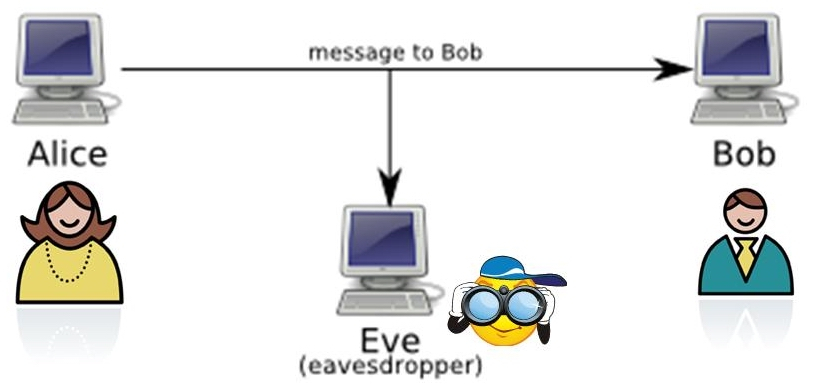
\includegraphics[scale=0.8]{./aliceBob.jpg}\end{center}
					\begin{exampleblock}{Problem of confidentiality}
						A message $M$ (plain text) has to be transmitted on a canal, but it could be intercepted. 
						\vspace*{5mm}
						
						The aim of cryptography is to prevent the attacker to be able to understand the message, or to exploit it in any way.
					\end{exampleblock}
				\end{frame}
				\subsubsection{Authentication and integrity}
				\begin{frame}
					\begin{exampleblock}{Problem of authentication and integrity}
						\begin{enumerate}
						
						\item authentication\footnote{authenticate : To establish the authenticity of; prove genuine} :  the message $M$ is coming from the right person
						\vspace*{8mm}
						\item integrity : $M$ hasn't be modified in any way.
						\vspace*{8mm}
						\end{enumerate}
					\end{exampleblock}
					\vspace*{10mm}
					When you connect to your bank, you wan't to be sure that it is really your bank you are connecting to, and you want to be sure the right amounts are transferred.
				\end{frame}
			\subsection{First example}
			\begin{frame}
				\begin{block}{Caesar cipher}
					Pick a number $n$ between 0 and 25 and then replace all letters of the message by the $n$-th letter after them (restarting at $A$ if necessary).
					\vspace*{10mm}
					
					For example $M= B$ with $n=3$ becomes $E$.
					 
					 $M = OUI$ with $n = 10$ becomes $YES$.
				\end{block}
					\vspace*{15mm}
					$n$ is called the \emph{key} of the cipher. It is a parameter in the encryption.
					\vspace*{8mm}
					
					The number of possible keys is called the \emph{keysize}.
			\end{frame}
			\subsection{Principles}
				\subsubsection{What is required for a cryptosystem}
				\begin{frame}
					
					\begin{block}{Kerckhoffs's principle}
						A cryptosystem should be secure even if everything about the system, except the key, is public knowledge.
					\end{block}
					\vspace*{5mm}
					Bad example : Enigma machines used by the Germans during World War 2%, its security relied in part on the fact the Allied didn't have any of the device used for encryption.
					
					\vspace*{5mm}
					You can't be sure of a non published algorithm.
					
					It is far more complicated to guess a random number (the key) than to find how a secret algorithm works.
					%If a key is compromised, you can roll a new one very easily.
				\end{frame}
				\begin{frame}	
					\begin{block}{Absolutely secure vs Computationally secure}
						\begin{itemize}
							\item absolutely secure : it is impossible to retrieve the plaintext without knowing the key.
								%Although there exist absolutely secure algorithms, they are of no practical use (they replace a hard problem, managing a message, by another hard problem : managing a key as long as the message)
								\vspace*{10mm}
							\item computationally secure : retrieving the plaintext without knowing the key won't be possible with many computational power before a long period of time %(this can be $10^{10}$ years).
						\end{itemize}
						
						
					\end{block}
					\vspace*{10mm}
					\begin{quote}If all the personal computers in the world - ~260 million computers - were put to work on a single PGP-encrypted message, it would still take an estimated 12 million times the age of the universe, on average, to break a single message.\end{quote}
					 William Crowell, Deputy Director of the National Security Agency, March 1997
				\end{frame}
				
				\subsubsection{Algorithmic complexity}
				\begin{frame}
					\begin{block}{What is complexity ?}
						Problems in computer sciences can be very easy or very hard :
						
						Easy problems : adding two integers, multiply two integers, finding the shortest path on a map between two points
						
						Hard problems : factoring integers, discrete logarithms
					\end{block}
					
					One measures complexity in number of elementary operations.
					\begin{itemize}
						\item Adding two $n$-bits integers is $O(n)$. Multiplying them is $O(n^2)$ and even $O(n \log n \log \log n)$.
						\item Factoring a random integer is $O(2^{n/2})$ or a bit better.
					\end{itemize}
					\vspace*{10mm}
					Trapdoor function : easy to compute the inverse if you know the secret. Very hard if you don't know it.
				\end{frame}
				\subsubsection{Symmetric cryptography}
				\begin{frame}
					A symmetric algorithm uses one key for both encryption and decryption. It is analogous to putting the message in a locked stash.
					
					The advantages : very fast encryption and decryption
					
					\begin{center}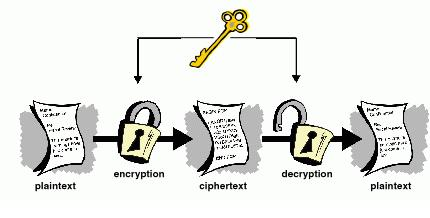
\includegraphics[scale=2]{./symmetric}\end{center}
					
					Main problem : \alert{how do you communicate the secret key ?}
				\end{frame}
				\subsubsection{Asymmetric cryptography}
				\begin{frame}
					Diffie–Hellman key exchange : an example of how you can safely exchange a key
					\begin{center}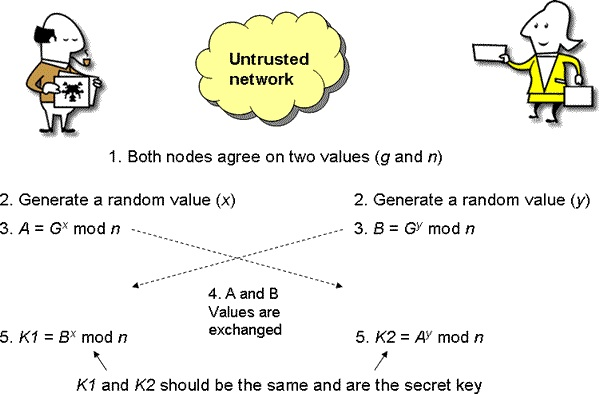
\includegraphics[scale=1]{./diffie1}\end{center}
				\end{frame}
				\begin{frame}
					\begin{block}{Public key cryptosystem}
						For such systems, there are two keys : one for encrypting, one for decrypting.
					\end{block}
					\begin{center}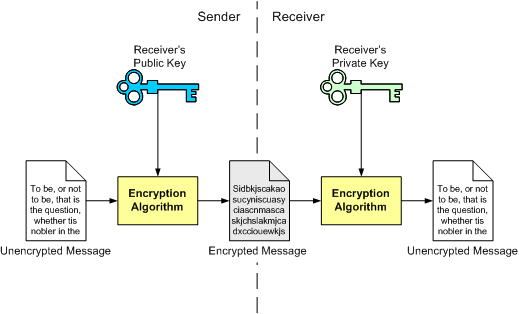
\includegraphics[scale=1.4]{./asymmetric}\end{center}
				\end{frame}
				\begin{frame}
					\begin{center}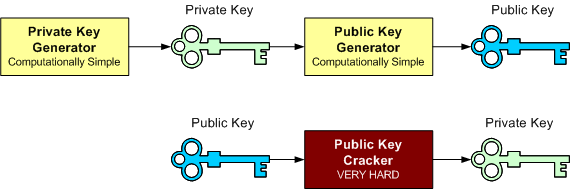
\includegraphics[scale=1.2]{./generation}\end{center}
				\end{frame}
				\begin{frame}
					Completing a public key cryptosystem with the precedent example :
					
					\begin{center}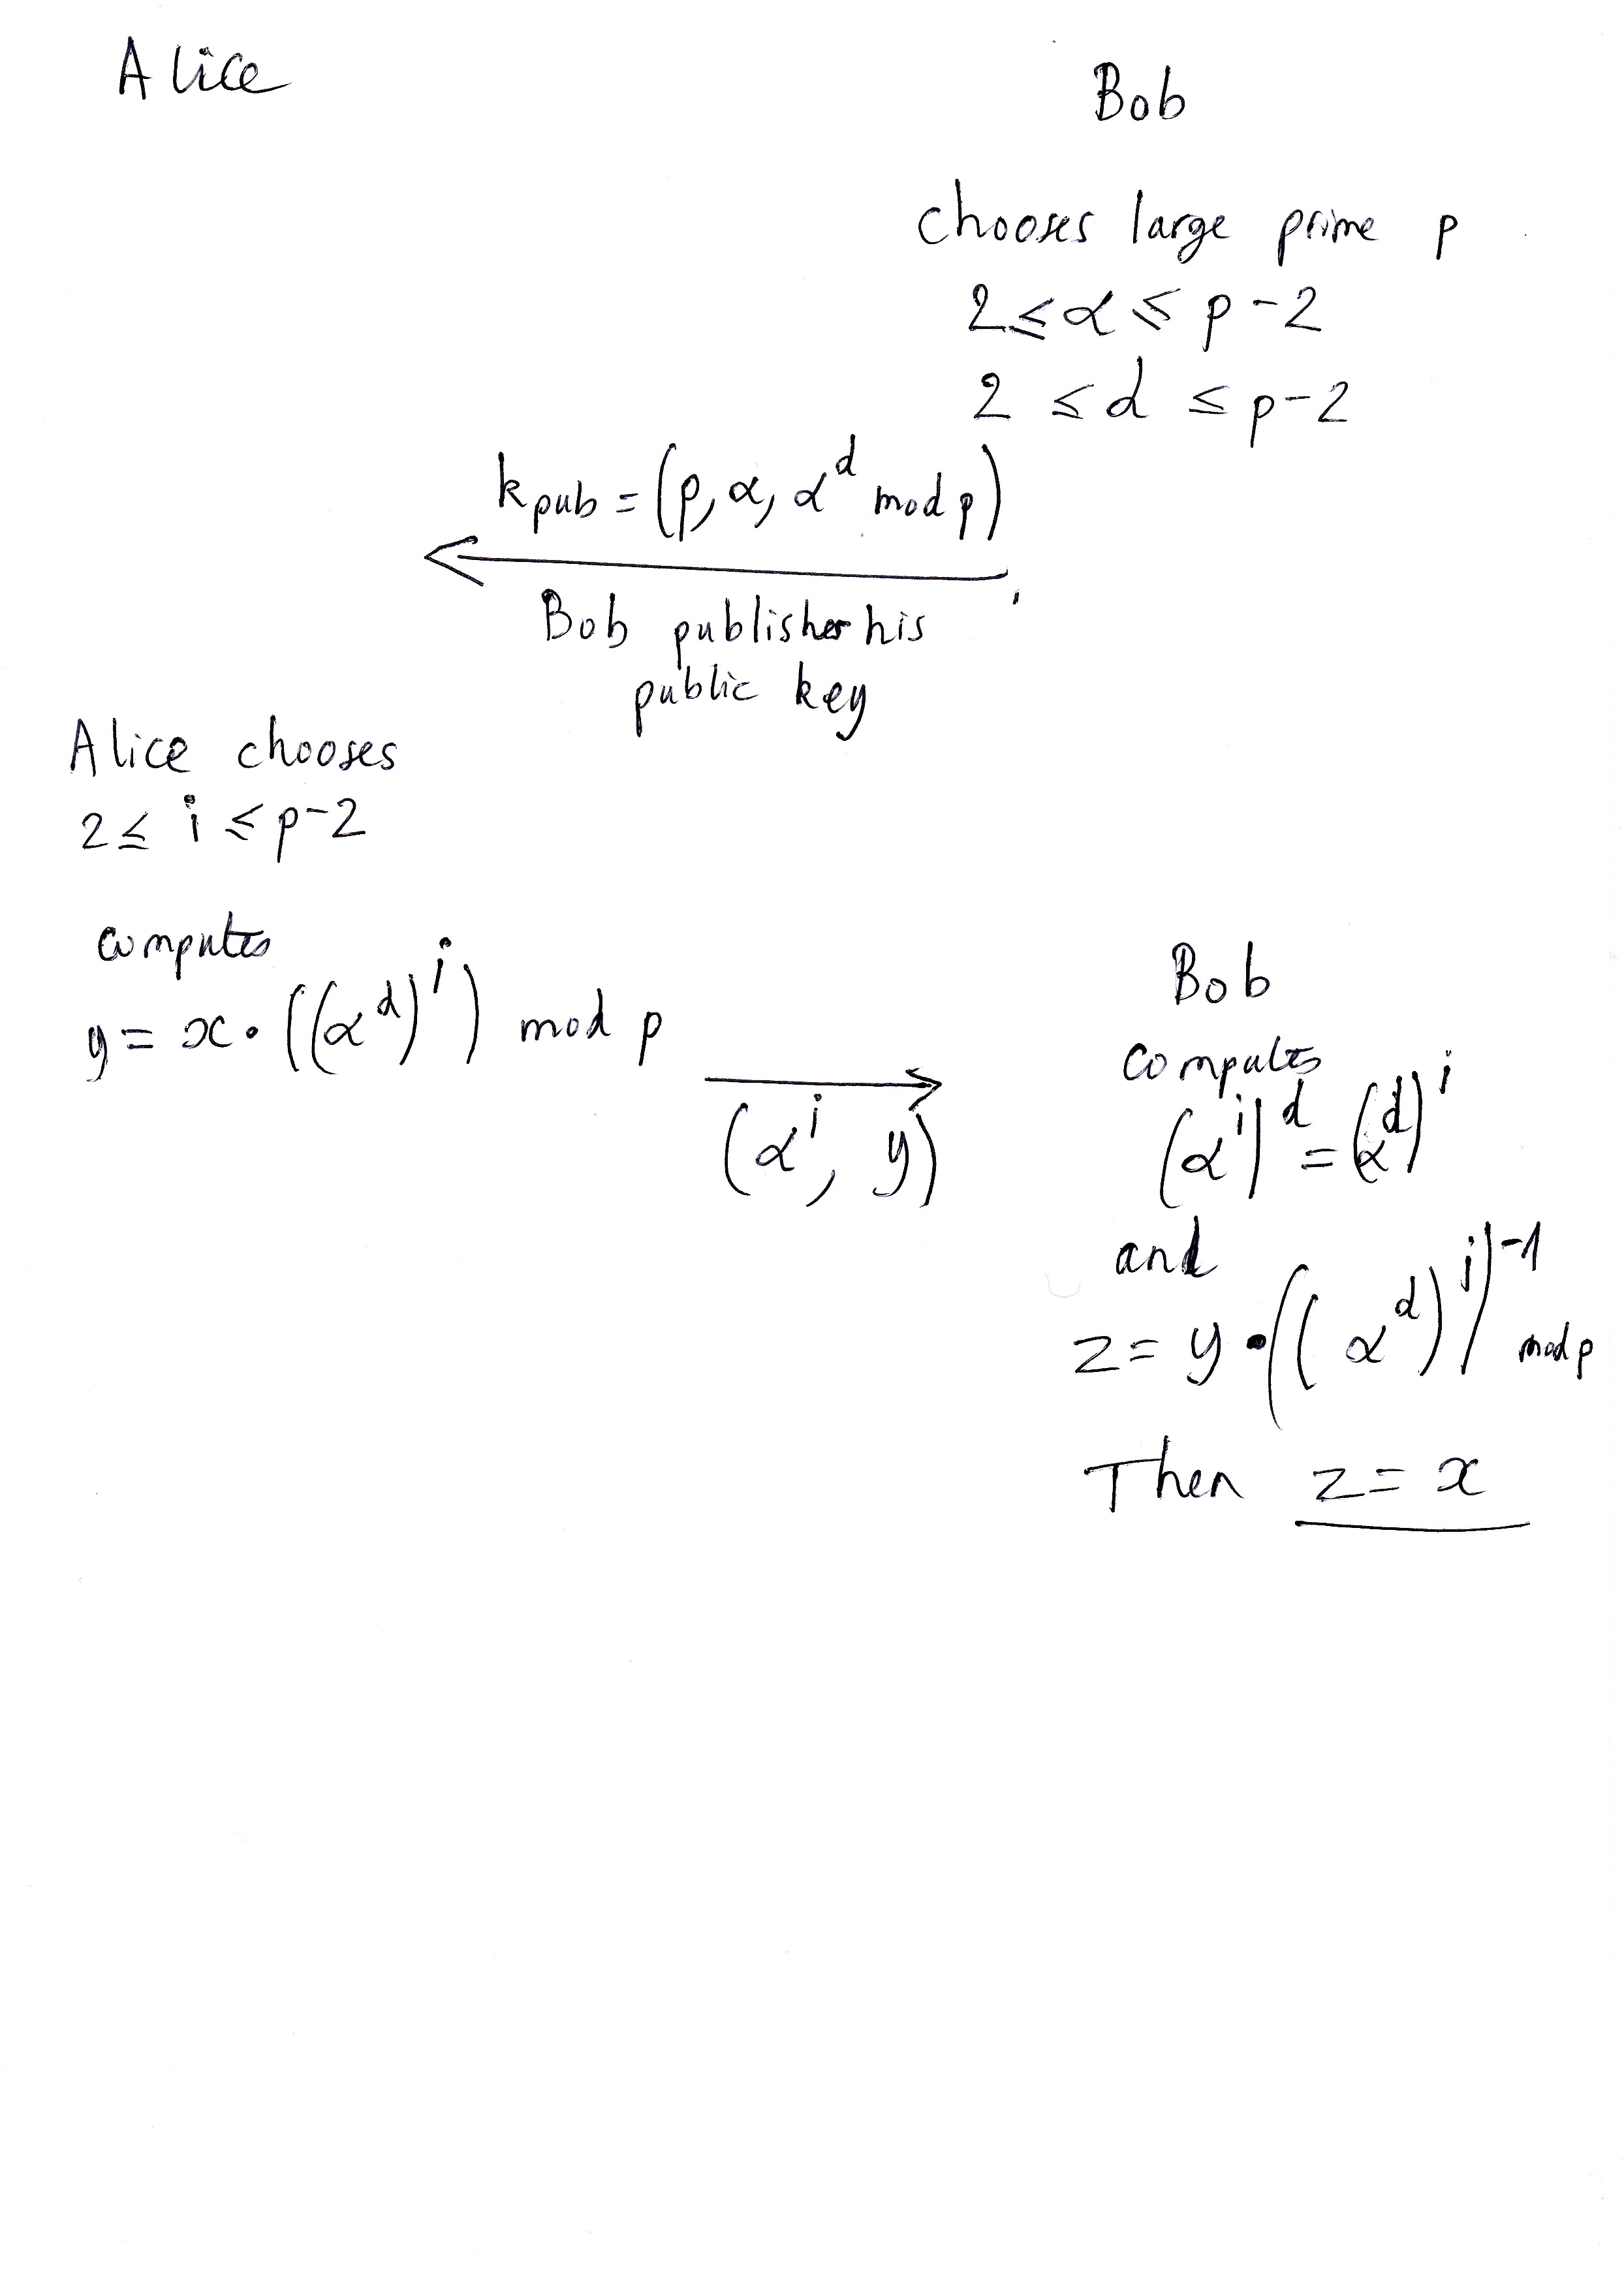
\includegraphics[scale=0.2]{./elgamal}\end{center}
				\end{frame}
				\begin{frame}
					\begin{center}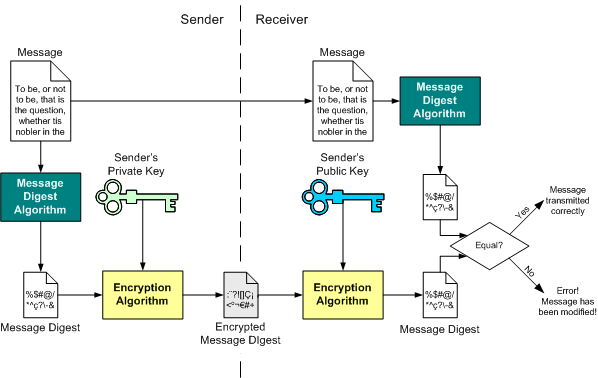
\includegraphics[scale=1.1]{./digitalsig}\end{center}
				\end{frame}
		\section{Practical usage}
			\subsection{Free software}
			\begin{frame}
				\begin{block}{On the importance of open source}
				\begin{itemize}
				\item Free software : the recipe or the code is public.
				\vspace*{10mm}
				
				\item You shouldn't ever trust closed source softwares. They offer you no guarantee on what is happening when they are working.
				
				US companies are putting backdoors in their softwares upon request by the NSA. (This isn't conspiracy theory, see \cite{scheneir},  \cite{nytcrypt} and \cite{greenwcrypt})
				\end{itemize}
				\end{block}
				%Examples : Skype (Microsoft), Windows.
			\end{frame}
			\subsection{Using encryption}
				\begin{frame}
					\begin{block}{A few practical advices}
					\begin{itemize}
						\item HTTPS : it is HTTP with encryption (public key algorithm)
					
							Use HTTPS everywhere plugin with your browser.
							\vspace*{10mm}
							
						\item Use PGP (pretty good privacy) for your emails whenever it is possible. (Download Thunderbird and Enigmail plugin).
						\vspace*{10mm}
						\item Encrypt your laptop's hard drive (or at least important files)
						\vspace*{10mm}
						\item For more information (phone encryption and so on), go to \url{https://prism-break.org}.
					\end{itemize}
					\end{block}
				\end{frame}
			%\subsection{Emails}
			%	\begin{frame}
			%		PGP : Use Thunderbird with the Enigmail plugin.
			%	\end{frame}
			%\subsection{Phone and instant messaging}
			%	\begin{frame}
			%	
			%	\end{frame}
		
%		\section{Question}
%			\begin{frame}
%			\alert{\emph{Objectif :}} Introduire quelques concepts d'analyse harmonique et fonctionnelle afin de présenter un théorème taubérien et une de ses conséquences arithmétiques.
%			\pause
%			\begin{block}{Késako ?}
%				\begin{itemize}[<+-| structure@+>]
%	  			\item Qu'est ce que l'analyse harmonique ?  C'est à une vache près l'analyse de Fourier.
%				
%				\item Qu'est que l'analyse fonctionnelle ? C'est l'étude des espaces de fonctions.
%				
%				\item Qu'est ce qu'un théorème taubérien ? C'est un théorème qui étant donnée une suite ou une fonction, en supposant la convergence d'une somme, d'une moyenne ou d'une convolée ainsi qu'une hypothèse supplémentaire appelée condition taubérienne, affirme la convergence d'une suite ou d'une fonction associée à la première.
%				\end{itemize}
%	 		\end{block}
%			\end{frame}
			

%					\begin{frame}
%			
%					\begin{alertblock}{Théorème taubérien de Wiener}
%						Soit $N\in L^1(\R) $, si $\widehat{N}$ ne s'annule pas et s'il existe $f\in L^{\infty}(\R) $ et $\ell \in \C $ tels que $ \lim_{x\rightarrow +\infty} N \ast f (x) = \ell \intex N(t) dt = \ell \hat{N}(0) $, alors pour tout $M\in L^1(\R) $ : \[ \lim_{x\rightarrow +\infty} M \ast f (x) = \ell \intex M(t) dt = \ell \hat{M}(0) \]
%					\end{alertblock}\pause
%					\begin{demo}
%						Soit $V$ l'ensemble des $M\in L^1(\R) $ tels que $\lim_{x\rightarrow +\infty} M \ast f (x) = \ell \intex M(t) dt$. Comme $V$ est non vide car il contient $N$, la linéarité à gauche de la convolution et la linéarité de la limite et de l'intégrale impliquent que $V$ est un sous-espace vectoriel de $L^1(\R)$. Or on voit immédiatement qu'il contient l'ensemble des translatées de $N$, en effet pour tout $a\in \R$, on a $N_a \ast f =(N \ast f)_a $. Donc il contient le sous-espace vectoriel engendré par les translatées de $N$, qui est quant à lui dense dans $L^1(\R )$. Par suite $V$ est dense, il suffit donc de montrer qu'il est fermé pour arriver à la conclusion, ce que l'on peut faire grâce à la caractérisation séquentielle de la limite. Soit donc $(M_n)_{n\in\N}$ une suite d'éléments de $V$ qui converge dans $L^1(\R)$ vers $M$.\end{demo}
%						\end{frame}
%						\begin{frame}
%						\begin{demo}[suite] Montrons que $M\in V$. Soit $\varepsilon > 0$ et $x \in \R $, il existe $n_0\in \N$ que $\| M_n - M\|_1 \le \frac{\varepsilon}{\| f \|_{\infty} +|\ell |+1} $ dès que $n \ge n_0$ on a :
%						\begin{align*}
%										\left| \conv{M}{f}(x) - \ell \intex M(t) dt \right| &\le \left| \conv{(M-M_n)}{f}(x)\right| + \left|\conv{M_n}{f}(x) - \ell \intex M_n(t) dt \right| \\
%																							&+ |\ell |\left|\intex (M_n(t) - M(t)) dt \right| \\
%										   													&\le \| M - M_n \|_{1} (\| f \|_{\infty} +|\ell |) + \left|\conv{M_n}{f}(x) - \ell \widehat{M}(0)\right| \\
%																   							&\le \varepsilon  + \left|\conv{M_n}{f}(x) - \ell \widehat{M}(0)\right|
%						\end{align*}
%						\end{demo}
%						\end{frame}
%						\begin{frame}
%							\begin{defi}[limites inférieure et supérieure]
%								Soit $f$ une fonction de $\R$ dans $\R $, on appelle respectivement limite inférieure et limite supérieure de $f$ les limites des fonctions monotones suivantes $x \mapsto \inf_{y\ge x} f(y)$ et $x\mapsto \sup_{y \ge x } f(y) $ et on note : 
%								\begin{align*}
%									\liminf_{x \rightarrow +\infty} f(x) &= \lim_{x \rightarrow +\infty}  \inf_{y\ge x} f(y) = \sup_x   \inf_{y\ge x} f(y)\\\
%									\limsup_{x \rightarrow +\infty} f(x) &= \lim_{x \rightarrow +\infty}  \sup_{y\ge x} f(y) = \inf_x   \sup_{y\ge x} f(y)
%								\end{align*}
%								Potentiellement on peut avoir la limite inférieure égale à $-\infty $ et/ou la limite supérieure égale à $+\infty$.
%							\end{defi}
%							\begin{theoreme}
%								$f$ admet une limite en $+\infty $ si et seulement si $\disp{\liminf_{x \rightarrow +\infty}f(x)=\limsup_{x \rightarrow +\infty}f(x) }$ et dans ce cas \[ \lim_{x \rightarrow +\infty}f(x) =\liminf_{x \rightarrow +\infty}f(x)=\limsup_{x \rightarrow +\infty}f(x) \]
%							\end{theoreme}
%							\begin{remarque}
%								Comme les limites supérieure et inférieure sont des limites, elles bénéficient des théorèmes de passage à la limite.
%							\end{remarque}
%						\end{frame}
%						\begin{frame}
%						\begin{demo}[suite]
%						On peut alors pour $n\ge n_0$ fixé passer à la limite supérieure lorsque $x$ tend vers l'infini, on obtient : \[ 0 \le \liminf_{x \rightarrow +\infty} \left| \conv{M}{f}(x) - \ell \intex M(t) dt \right| \le \limsup_{x \rightarrow +\infty} \left| \conv{M}{f}(x) - \ell \intex M(t) dt \right| \le \varepsilon \] car $\lim_{x \rightarrow +\infty} \left| \conv{M_n}{f}(x)- \ell \widehat{M_n}(0) \right| = 0$. D'où puisque $\varepsilon $ est arbitrairement petit, \[ \lim_{x \rightarrow +\infty} \left| \conv{M}{f}(x)- \ell \intex M(t) dt \right| = 0 \] Cela revient exactement à dire que $M \in V$, d'où la conclusion.
%					\end{demo}
%					\pause Le théorème taubérien de Wiener permet sous l'hypothèse de non-annulation de la transformée de Fourier, de remplacer une noyau de convolution donné par n'importe quel noyau.
%					\end{frame}
%	
%				\begin{frame}
%					Les fonctions arithmétiques, qui sont par définition des fonctions de $\N^ * $ dans $\C $ vont constituer notre pont entre l'analyse et l'arithmétique. Grâce à leur étude asymptotique, on va pouvoir utiliser l'arsenal des théorèmes taubériens, nous donnant ainsi accès au théorème des nombres premiers. Le théorème des nombres premiers utilise la fonction $\disp{\pi : x \mapsto \textrm{card} \{ p\in\P / p \le x\}= \sum_{p \le x } 1}$.
%					\begin{defi}[fonctions de Von Mandgoldt et de Tchebychev]
%						On note $\Lambda $ la fonction de $\N^* $  dans $\R $ qui à $n$ associe $\ln p $ si $n = p^m $ avec $p$ premier et $m\in\N^* $ et $0$ sinon.
%						On note alors $\psi : x \mapsto \sum_{1 \le k \le x} \Lambda(k) = \sum_{2\le p^m \le x} \ln p $.
%					\end{defi}
%					La proposition suivante montre que le théorème des nombres premiers est une conséquence de $\psi( x )\sim x $ lorsque $x$ tend vers $+\infty $.
%					\begin{proposition}
%						On a pour tout $x > e $ : \[ \frac{\psi (x)}{x} \le \pi(x)\frac{ \ln x}{x} \le \frac{\psi (x)}{x}\cdot\frac{1}{1 - 2\frac{\ln\ln x}{\ln x}}+ \frac{1}{\ln x} \]
%					\end{proposition}
%					\end{frame}
%					\begin{frame}
%					\begin{demo}
%						Démontrons la première inégalité. On a pour tout $x > e$, \[\psi(x) = \sum_{2 \le p^m \le x} \ln p = \sum_{p\le x} \left\lfloor \frac{\ln x}{\ln p} \right\rfloor \ln p \le \ln x \sum_{p\le x} 1 =\pi(x)\ln x\] En effet entre $2$ et $x$, il y a $\lfloor \log_{p} x \rfloor $ puissances de $p$, pour $p$ premier. En divisant par $x$ on obtient l'inégalité voulue.
%	
%						Démontrons la seconde inégalité. Soit $x$ et $y$ avec $e< y < x$. On a \[ \pi(x) - y \le \pi(x) - \pi(y) = \sum_{y< p \le x} 1 \le \sum_{y< p \le x} \frac{\ln p}{\ln y} \le  \frac{1}{\ln y}\sum_{p \le x} \ln p \le \frac{\psi(x)}{\ln y}\] En posant $y = \frac{x}{\ln^2 x}$, on obtient 
%						\begin{align*}
%							\pi (x) &\le \frac{x}{\ln^2 x} + \frac{\psi(x)}{\ln \frac{x}{\ln^2 x}}\\
%							\pi(x)\frac{ \ln x}{x}& \le  \frac{1}{\ln x}+ \frac{\psi (x)}{x}\cdot\frac{\ln x}{\ln x - 2 \ln\ln x}
%						\end{align*} 
%						La deuxième inégalité en découle immédiatement.
%					\end{demo}
%					\end{frame}
%					\begin{frame}
%						\begin{proposition}
%							Soit $F : x \mapsto \sum_{n = 1}^\infty \psi(\frac{x}{n})$, on a lorsque $x$ tend vers $+ \infty$ \[F(x) = x\ln x - x + O(\ln x) \]
%						\end{proposition}
%						\begin{demo}
%							On remarque que $F$ est constante par morceaux.
%							Montrons que pour tout $n\in\N^*$, $F(n) = \ln n\,!$. Soit $n\in\N^* $, on \[ F(n)-F(n-1)=\sum_{k=1}^{+\infty} \psi\left(\frac{n}{k}\right)-\psi\left(\frac{n-1}{k}\right) = \sum_{k|n} \Lambda\left(\frac{n}{k}\right) =\sum_{d|n} \Lambda(d) = \ln n  \] La dernière étape est une conséquence du théorème fondamental de l'arithmétique.
%							
%							On a alors pour $x\ge 1 $, $F(x) = \ln\left( \lfloor x \rfloor !\right)$. D'où par comparaison entre la série $(\sum_{k=1}^n\ln k )_n$ et la fonction $x\mapsto \int_{[1;\, x]}\ln t \,dt$,  on a $F(x)=x\ln x - x + O(\ln x)$ lorsque $x$ tend vers l'infini.
%						\end{demo}
%					\end{frame}
%	    
%					\begin{frame}
%					La fonction $\zeta $ de Riemann et plus généralement les fonctions $L$ sont un des outils principaux de la théorie analytique des nombres. On va voir que le simple fait que la fonction $\zeta $ ne s'annule pas sur la droite des complexes de partie réelle 1 suffit à démontrer le théorème des nombres premiers.
%					\begin{defi}[fonction $\zeta$ de Riemann]
%					 	Soit $\zeta $ la fonction\footnote{Cette fonction est bien définie car la série associée est absolument convergente.} de l'ensemble des complexes de partie réelle strictement supérieure à $1$ dans $\C $ qui à $s$ associe $\disp{\sum_{k=1}^{+\infty} \frac{1}{k^s}}$. 
%					\end{defi}
%					\begin{proposition}[produit eulérien]
%						On a pour tout complexe $s$ avec $\Re s > 1$ : \[ \zeta(s) = \prod_{p \textrm{ premier}} \frac{1}{1 - p^{-s}} \]
%					\end{proposition}
%					\end{frame}
%					\begin{frame}
%						\begin{proposition}[formule d'Abel]
%							Soit $(u_n)_{n\ge 1}$ une suite complexe, $x\in [ 1 ; +\infty [$ et $v\in \mathcal{C}^1([1; x ],\R)$. En posant pour tout réel $t\ge 1$, $U(t) = \sum_{1\le n \le t} u_n$, on a \[ \sum_{1\le n \le x} u_n v(n) = U(x)v(x) - \int_{[1;\,x]} U(t)v'(t)dt\]
%						\end{proposition}%\vspace*{3mm}
%					\begin{theoreme}[prolongement de $\zeta $]
%						On peut étendre $\zeta $ à l'ensemble des complexes s avec $\Re s > 0$ privé de $1$, elle est encore holomorphe\footnote{Elle est dérivable au sens complexe.} et est définie par l'expression \[ \zeta(s) = \frac{s}{s-1}+s\int_{[1 ; +\infty [} \frac{\left\{u \right\}}{u^{s+1}}du \]
%					\end{theoreme}
%					\begin{block}{Indication}
%						C'est une simple application de la formule de sommation d'Abel pour les intégrales suivie d'un passage à la limite.
%					\end{block}
%					\end{frame}
%					\begin{frame}
%						\frametitle{Non annulation de $\zeta $ sur la droite complexe $\Re s = 1$}
%						Deux des avantages de la démonstration du TNP par les théorèmes taubériens est qu'elle n'exige ni d'étendre $\zeta $ à tout le plan complexe, ni de montrer que $\zeta $ ne s'annule pas sur une petite bande autour de la droite $\Re s = 1$.
%						\begin{alertblock}{Théorème de La Vallée Poussin-Hadamard}
%							Pour tout $t\in \R^*$, \[ \zeta(1+it) \neq 0 \]
%						\end{alertblock}
%						\begin{block}{Indication}
%							On suppose qu'il existe un zéro $z\in\C \textbackslash{}\{ 1\}$ de $\zeta $ avec $\Re z = 1$. On prend une détermination principale du logarithme et on l'applique au produit eulérien. On obtient une inégalité\footnote{Sur des modules !} pour tout complexe $s$ tel que $\Re s > 1$ et on obtient une contradiction en passant à la limite quand $\Re s$ tend vers 1.
%						\end{block}
%					\end{frame}
%		
%					\begin{frame}	
%					\begin{alertblock}{Théorème taubérien d'Ingham}
%						Soit $f : ]0; \infty[\to \R$, croissante et telle que $f(x) = 0$ si $0< x < 1$. Soit $F : x \mapsto \sum_{k = 1}^\infty f( \frac{x}{k} )$.
%	S'il existe $a$ et $b$ dans $\R$ tels que $F(x)=a\cdot x\ln x+b\cdot x+o(x)$ lorsque  $x$ tend vers $+\infty$, alors \[\lim_{x \rightarrow +\infty} \frac{f(x)}{x} = a \]
%						\label{ingham}
%					\end{alertblock}
%					\begin{block}{Schéma de la preuve}
%						On démontre tout d'abord que $g: x\mapsto x^{-1}f(x)$ est bornée grâce à une somme télescopique.
%						
%						Puis l'on pose une fonction $K$ dont la transformée de Fourier est égale sur $\R^*$ à $t\mapsto \zeta(1+it)$ multipliée par une fonction qui ne s'annule pas. On peut alors appliquer le théorème de Wiener à $g$ pour obtenir que pour tout $\varepsilon >0$, \[ a\cdot e^{-\varepsilon} \le \varliminf_{x\rightarrow +\infty} g(x) \le  \varlimsup_{x\rightarrow +\infty} g(x) \le a\cdot e^{\varepsilon} \]
%						Par suite $g$ admet $a$ pour limite en $+\infty $.
%					\end{block}
%					\end{frame}
%		
%				\begin{frame}
%				Le théorème des nombres premiers donne une évaluation asymptotique du cardinal de l'ensemble des nombres premiers entre $0$ et $x\in\R$. 
%				\begin{alertblock}{TNP}
%					On a lorsque $x$ tend vers $+\infty $ \[ \pi (x) \sim \frac{x}{\ln x} \]
%				\end{alertblock}
%				\begin{demo}
%					Comme on l'a déjà vu, ceci revient à démontrer que $\psi(x) \sim x$. Or d'après le théorème d'Ingham appliqué à la fonction $F:x\mapsto \sum_{k = 1}^{+\infty}\psi (\frac{x}{k}) $, qui on le rappelle vérifie $F(x) = 1\cdot x\ln x -x + O(\ln x )$ lorsque $x$ tend vers $+\infty $, on a $\disp{\lim_{x \rightarrow +\infty}x^{-1}\psi(x) = 1}$.
%				\end{demo}
%		\end{frame}
%		\begin{frame}
%		\section*{Conclusion}
%			\begin{exampleblock}{Conclusion}
%			Ainsi de pures considérations d'analyse harmonique et fonctionnelle peuvent aboutir à des théorèmes fondamentaux d'arithmétique.
%			
%			On peut ainsi démontrer le théorème de la progression arithmétique grâce à des théorèmes taubériens que l'on applique à des fonctions $L$\footnote{Généralisations de la fonction $\zeta $.}.
%			
%			Cependant les termes d'erreurs que permettent d'atteindre les théorèmes taubériens sont médiocres comparés à ceux obtenus par l'analyse complexe. Toutefois ils fournissent un accès simple au TNP\footnote{Le théorème taubérien de Newman portant sur la transformée de Laplace est une des voies les plus rapides vers le TNP.}.
%			\end{exampleblock}
%		\end{frame}
%		\section*{Annexe}
%			\subsection*{La théorie de Gelfand}
%				\label{gelfand}
%				\begin{frame}
%				\frametitle{Vers une preuve du théorème d'approximation de Wiener}
%					Il existe plusieurs démonstrations du théorème de Wiener. La prise en compte du caractère algébrique du problème s'avère très fructueuse. Ainsi un sous-espace de $L^1(\R)$ invariant par translation et fermé est un idéal. 
%					
%					La théorie de Gelfand permet d'étudier le problème de façon algébrique. En effet $L^1(\R)$ est une algèbre de Banach pour la convolution. On peut alors plonger $L^1(\R)$ dans une algèbre unitaire dont il est un idéal maximal. Comme la théorie de Gelfand établit une correspondance bijective entre les idéaux maximaux d'une algèbre de Banach unitaire et commutative et ses morphismes à valeurs dans $\C $, on a une caractérisation de l'inversibilité. Quelques manipulations algébriques et quelques considérations analytiques montrent alors que l'idéal engendré par $f$ contient l'ensemble des éléments de $L^1(\R)$ dont la transformée de Fourier est à support compact, lui-même dense dans $L^1(\R)$.
%				\end{frame}
				
		
		\nocite{*}
		\bibliographystyle{alpha} % Le style est mis entre crochets.
	         \bibliography{bibli}
	         \section*{Conclusion}
				\begin{frame}
					\huge{How much do you care about privacy ?}
					
					 Would you use cryptography ?
				\end{frame}
	\end{document}
